\documentclass[oneside,a4paper,11pt,explicit]{book}
\usepackage[utf8]{inputenc}
\usepackage{icecream}
\usepackage[english]{babel}
\addto\captionsenglish{\renewcommand{\chaptername}{}}
\usepackage[accsupp]{axessibility}  % improves PDF readability for those with disabilities.
\usepackage[colorlinks = true,urlcolor  = blue,linkcolor = blue]{hyperref}
\usepackage{setspace}
\usepackage{listings}
\usepackage[most]{tcolorbox}
\usepackage{minitoc}
\usepackage{multicol}


\renewcommand{\mtifont}{\large\sffamily}
\renewcommand{\mtcfont}{\small\sffamily}
\renewcommand{\mtcSfont}{\small\sffamily}
\renewcommand{\mtcSSfont}{\small\sffamily}
\renewcommand{\mtcSSSfont}{\small\sffamily}
\mtcsetpagenumbers{minitoc}{off} % turn off page numbering in minitocs
\addto{\captionsenglish}{% Making babel aware of special titles
	\renewcommand{\mtctitle}{Quick Links To Sections}
}
\setlength{\fboxrule}{5pt}
\setlength{\fboxsep}{4pt}

\definecolor{IceCreamLeaf}{HTML}{58743b}
\definecolor{IceCreamOrbit}{HTML}{732e00}
\definecolor{MACred}{rgb}{0.803921568627451, 0.3607843137254902, 0.3607843137254902}

\title{I.C.E.C.R.E.A.M. Tutorials}
\subtitle{\small Observing Earth from Above (Env 329) v24.06 \\
	\small Schmid College of Science and Technology, Chapman University}
\date{\today}

%% DOCUMENT
\setstretch{1.25}
\makeatletter
\begin{document}

\setcounter{tocdepth}{3}
\setcounter{minitocdepth}{3}
\dominitoc
\faketableofcontents

\setcounter{chapter}{0} %Insert (Tutorial Number-1) Here; example for tutorial 4, enter 3

\chapter{Installing QGIS} %Enter Tutorial Name Here

\vspace{-2em}

\minitoc

\hrule

\vspace{1em}

\begin{tcolorbox}[enhanced,frame style image=blueshade.png,
	opacityback=0.75,opacitybacktitle=0.25,
	colback=blue!5!white,colframe=blue!75!black,title={\Large \textbf{Objectives:}}]
	\large
	\begin{enumerate}
		\item Recognize geospatial data as information connected to a location.
        \item Install a geographic information system software called QGIS. 
        \item Consider the elements of effective maps. 
	\end{enumerate}
\end{tcolorbox}

\clearpage

%%%%%%%%%%%%%%%%%%%%%%%%%%%%%%%%%% Change Header to Have a Smaller Logo for Remainder of the Document
\fancyhead{}
\fancyhead[C]{\begin{tikzpicture}[overlay, remember picture]
		\fill[Blue2] (current page.north west) rectangle ($(current page.north east)+(0,-1in)$);
		\node[anchor=north west, text=white, font=\Large, minimum size=1in, inner xsep=5mm, align=left] at (current page.north west) {\bf{\MakeUppercase{\@title}}\\\@subtitle};
		\node[anchor=north east, minimum size=1in, inner xsep=5mm] at (current page.north east) {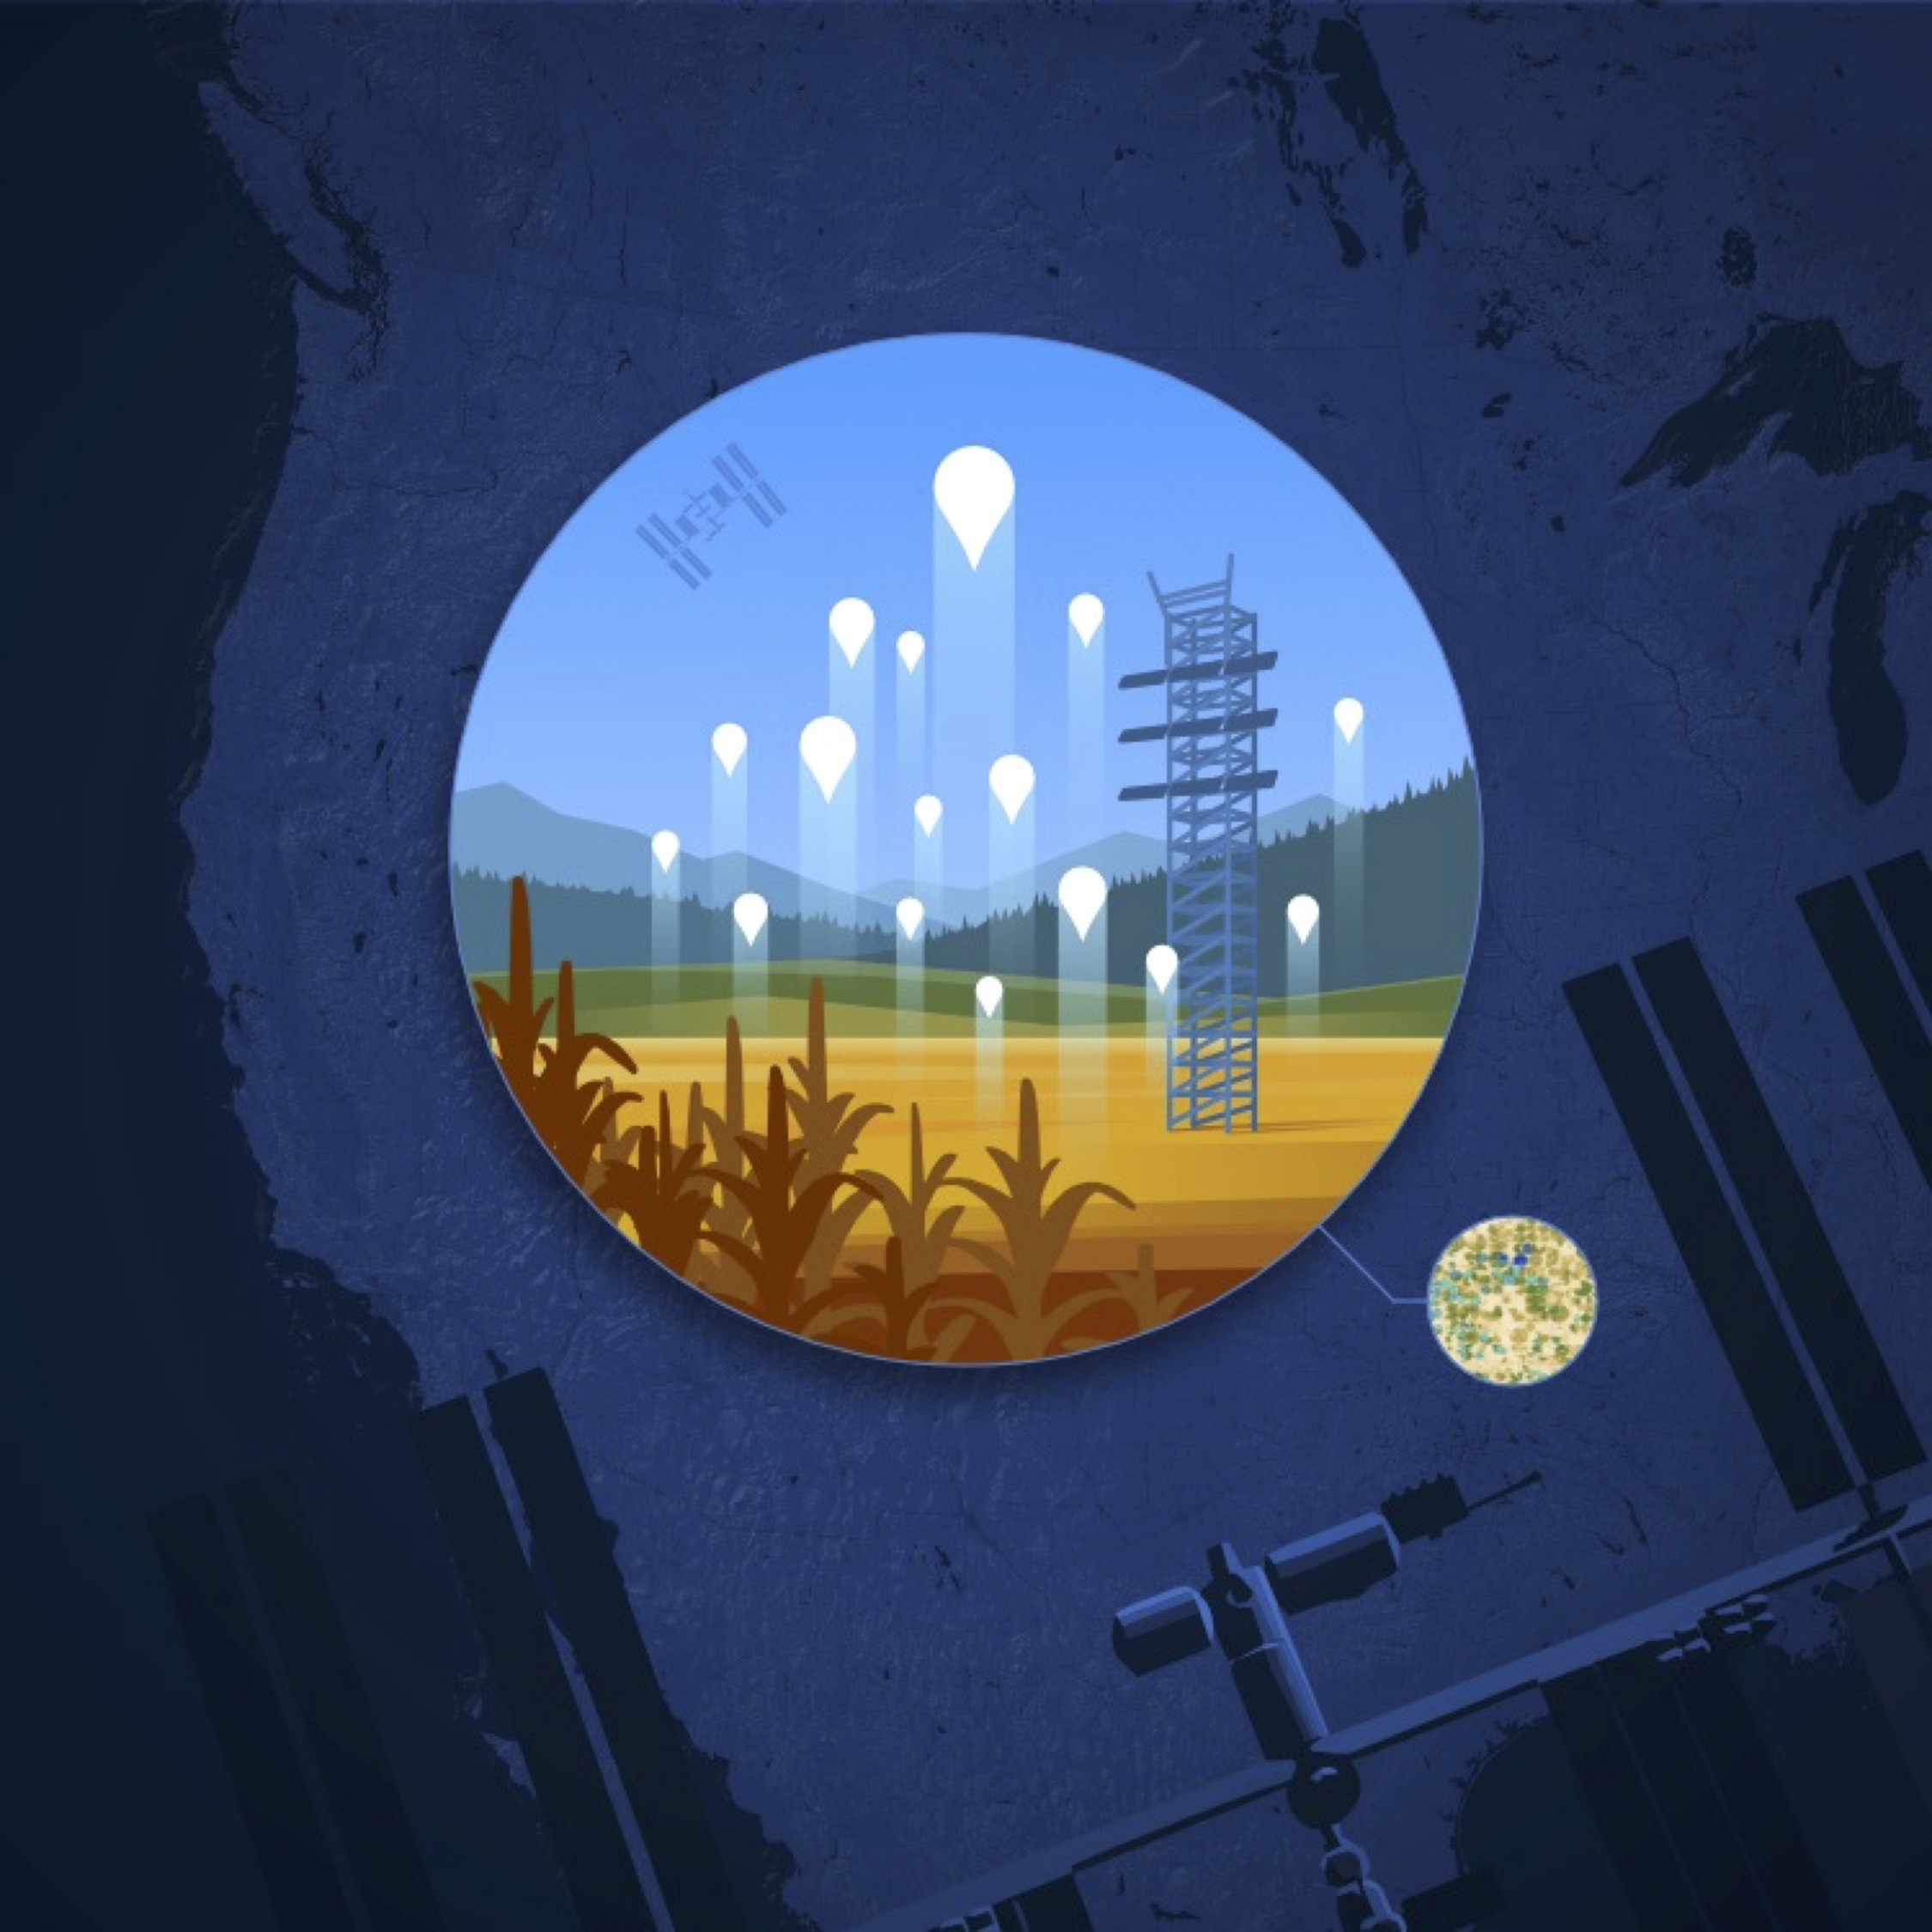
\includegraphics[scale=.03]{ECOSTRESS-BASE.jpg}};\end{tikzpicture}}
%%%%%%%%%%%%%%%%%%%%%%%%%%%%%%%%%%

\section{What is QGIS? Why Do I Need It?}

Geospatial data are any data that are connected to a specific location. Geospatial data can refer to objects, events, and other real-world phenomena that are related to a geographic area identified by latitude and longitude. We use data like this everyday when we navigate to museums, restaurants, or a friend's house using maps on our cellphones. In this course, we are going to analyze geospatial data from satellite remote sensing instruments and create maps that visualize environmental events (e.g., natural disasters or weather events). 

When we work with geospatial data, we refer to the system that organizes, analyzes, and visualizes those data as a geographic information system (GIS). QGIS is a GIS software program that supports viewing, editing, printing, and analyzing geospatial data.  If you have ever worked with GIS software before, you might have used a software program called ArcGIS. QGIS is a free and open source alternative to ArcGIS that is widely used in government, industry, and academic settings. Increasingly, researchers are also turning to programming languages (e.g., R and Python) and writing code to process and analyze geospatial data; however, the advantage of QGIS and ArcGIS is that they are menu-driven software programs. 

In each class, you will use QGIS to complete new tutorials and occasionally submit ``Make a Map'' assignments that will give you practice working with geospatial data and add new tools to your skill set. 

\section{Installing QGIS}

\kulbox{\textbf{NOTE:} QGIS requires 2 GB of storage on average and can take as much as 3 GB for a full install. 

\vspace{.5em}

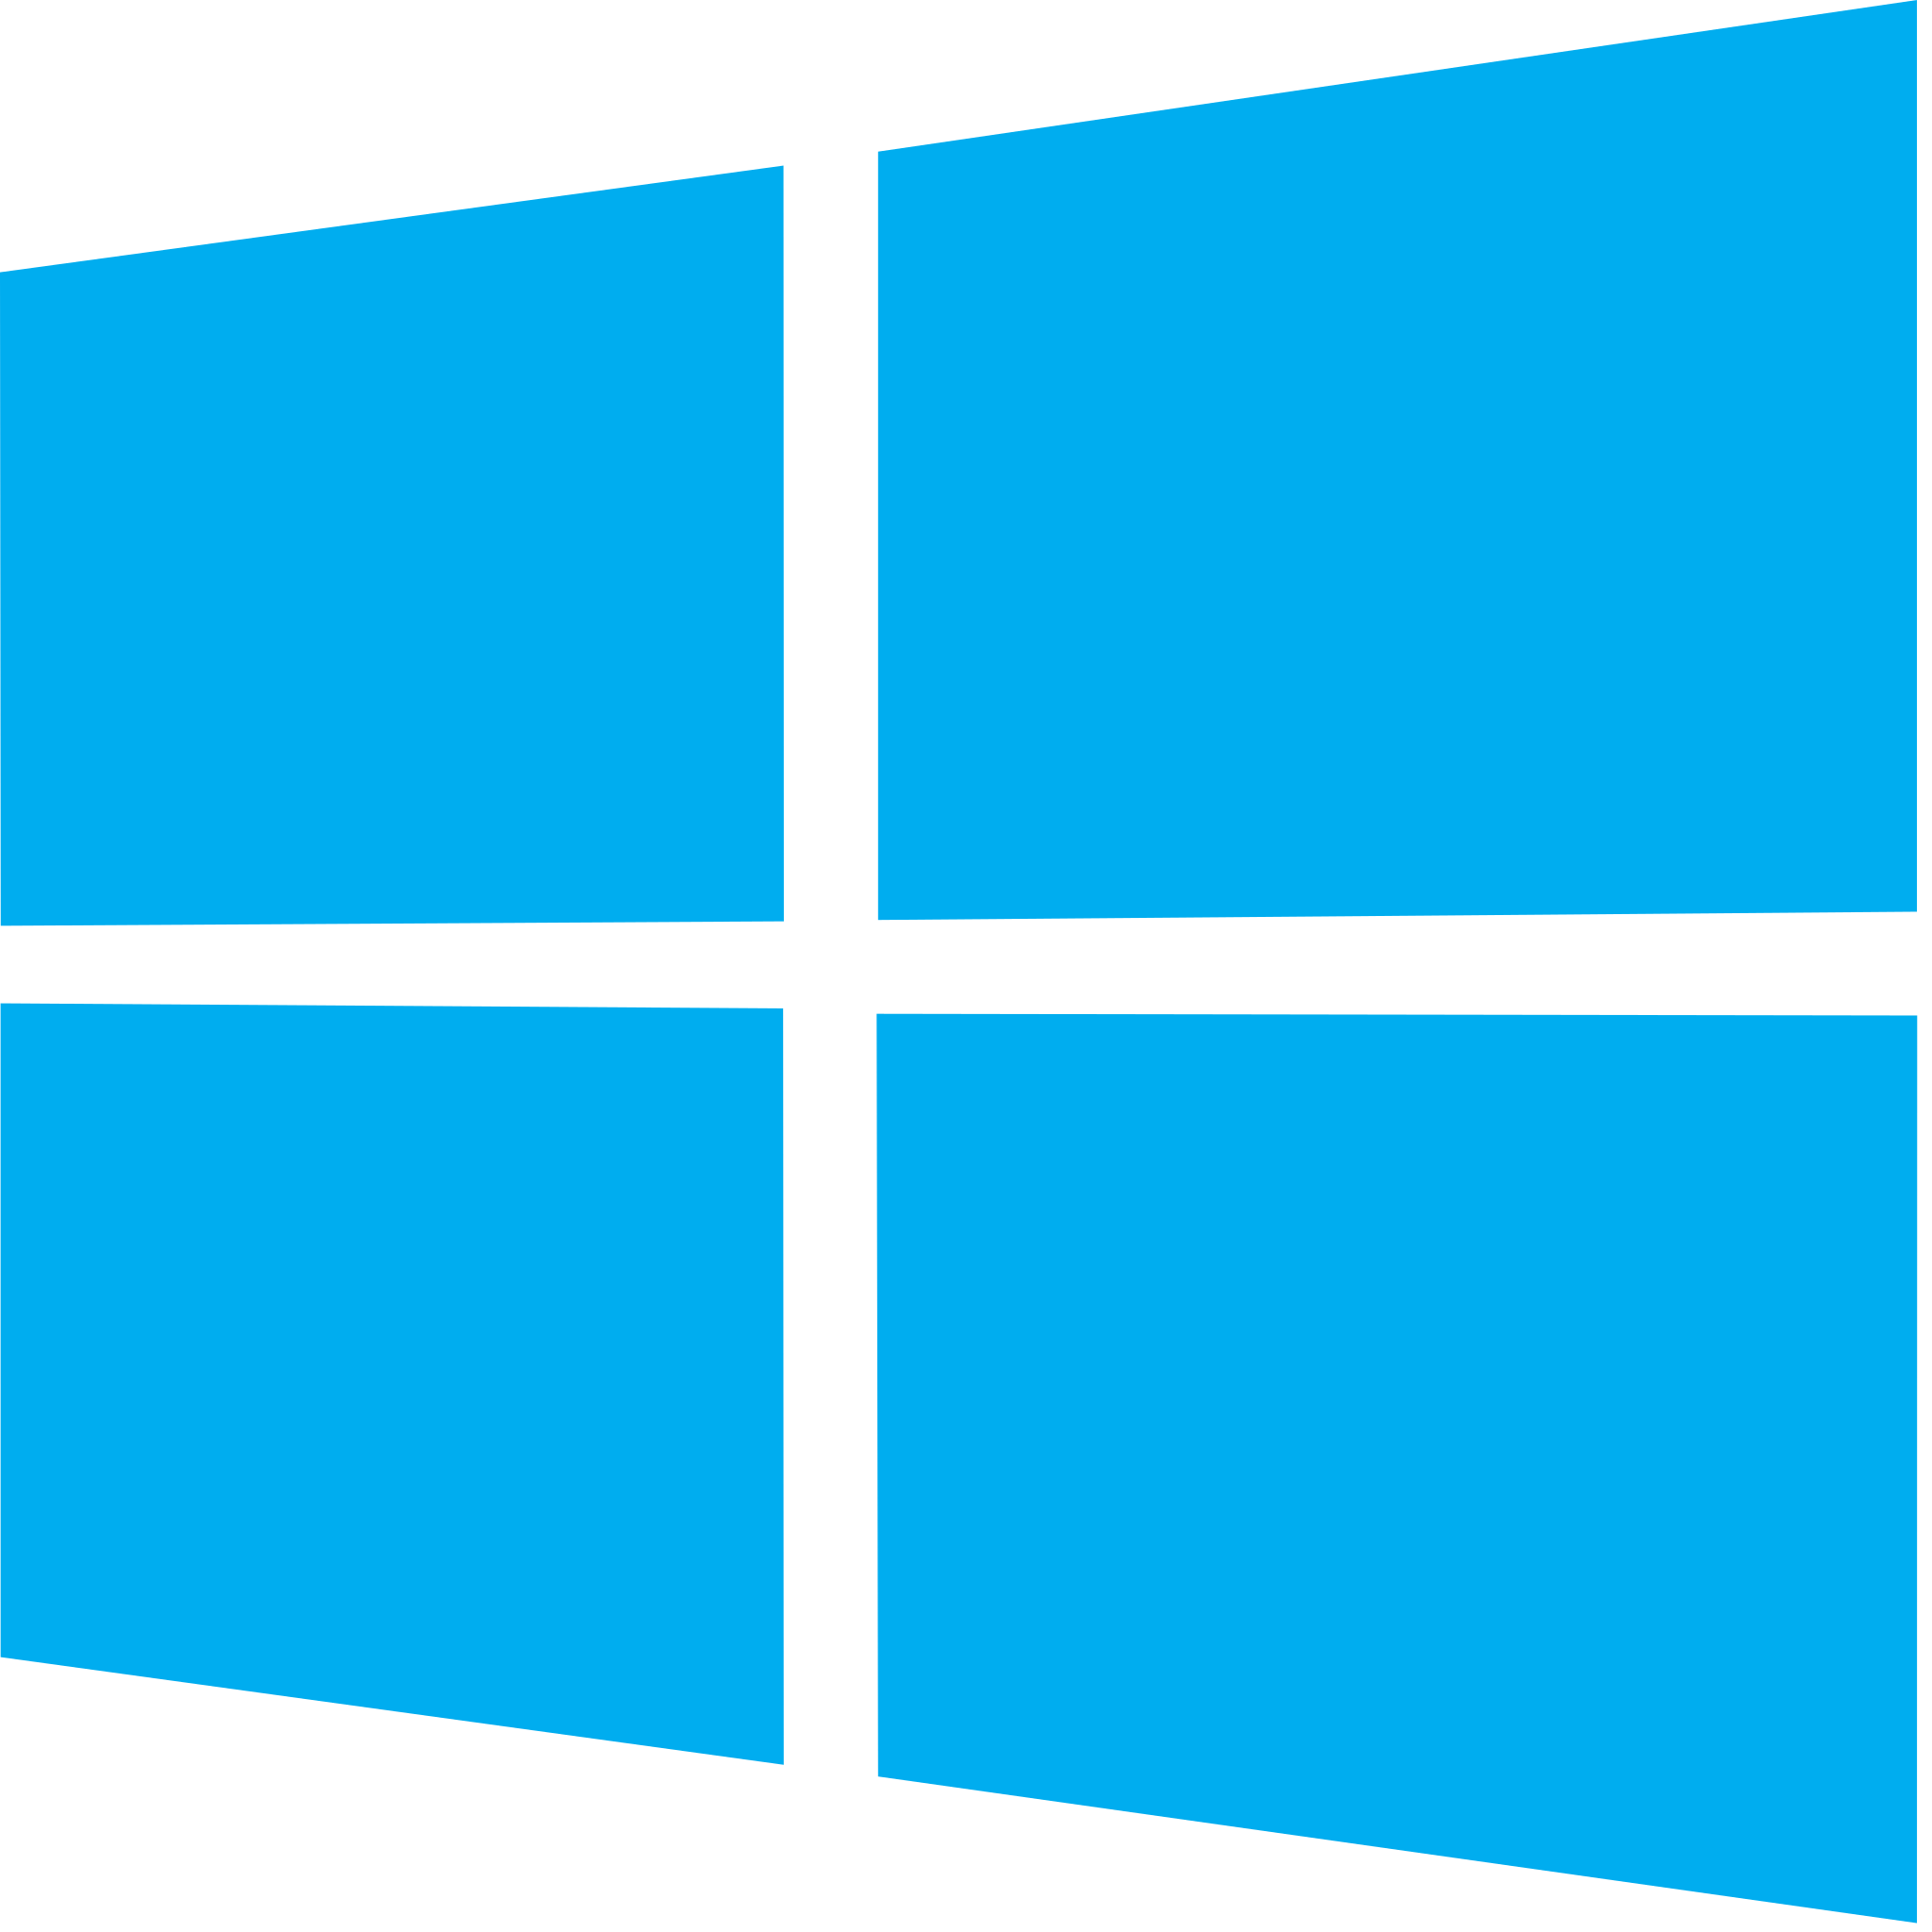
\includegraphics[width=.5cm]{WindowsLogo.png} To check your storage on Windows go to Start $\rightarrow$ Settings $\rightarrow$ System $\rightarrow$ Storage. 

\vspace{.5em}


\includegraphics[width=.5cm]{AppleLogo.png} On Mac, choose the Apple menu $\rightarrow$ System Settings $\rightarrow$ General $\rightarrow$ Storage}

1. Head over to \href{https://qgis.org/en/site/forusers/download.html}{https://qgis.org/en/site/forusers/download.html} and download the stable version of QGIS for your operating system (e.g., Mac, Windows, or Linux). If you already have another version of QGIS installed, we recommend that you update to the latest stable version so that your screen matches the tutorials.

\kulbox{\textbf{NOTE:} QGIS offers a "latest release" of its software which is cutting edge and unstable. We suggest downloading the Long Term Release (LTR), which is stable and easier to use. See images below for each operating system:}

\begin{tcolorbox}[colback=yellow!5!,title=\flushright{Linux \hspace{.25em} 
\includegraphics[width=1cm]{LinuxLogo.png}}]
	\begin{enumerate}
		\item Use your package manager to install the stable version from your distribution's repository or follow these instructions to install a more up-to-date version : \href{https://www.qgis.org/en/site/forusers/alldownloads.html#linux}{https://www.qgis.org/en/site/forusers/alldownloads.html\#linux}
		\item Open QGIS by selecting it in your applications launcher.
	\end{enumerate}
\end{tcolorbox}

\begin{tcolorbox}[colback=yellow!5!white,colframe=blue!60!green,title=\flushright{Windows \hspace{.25em} 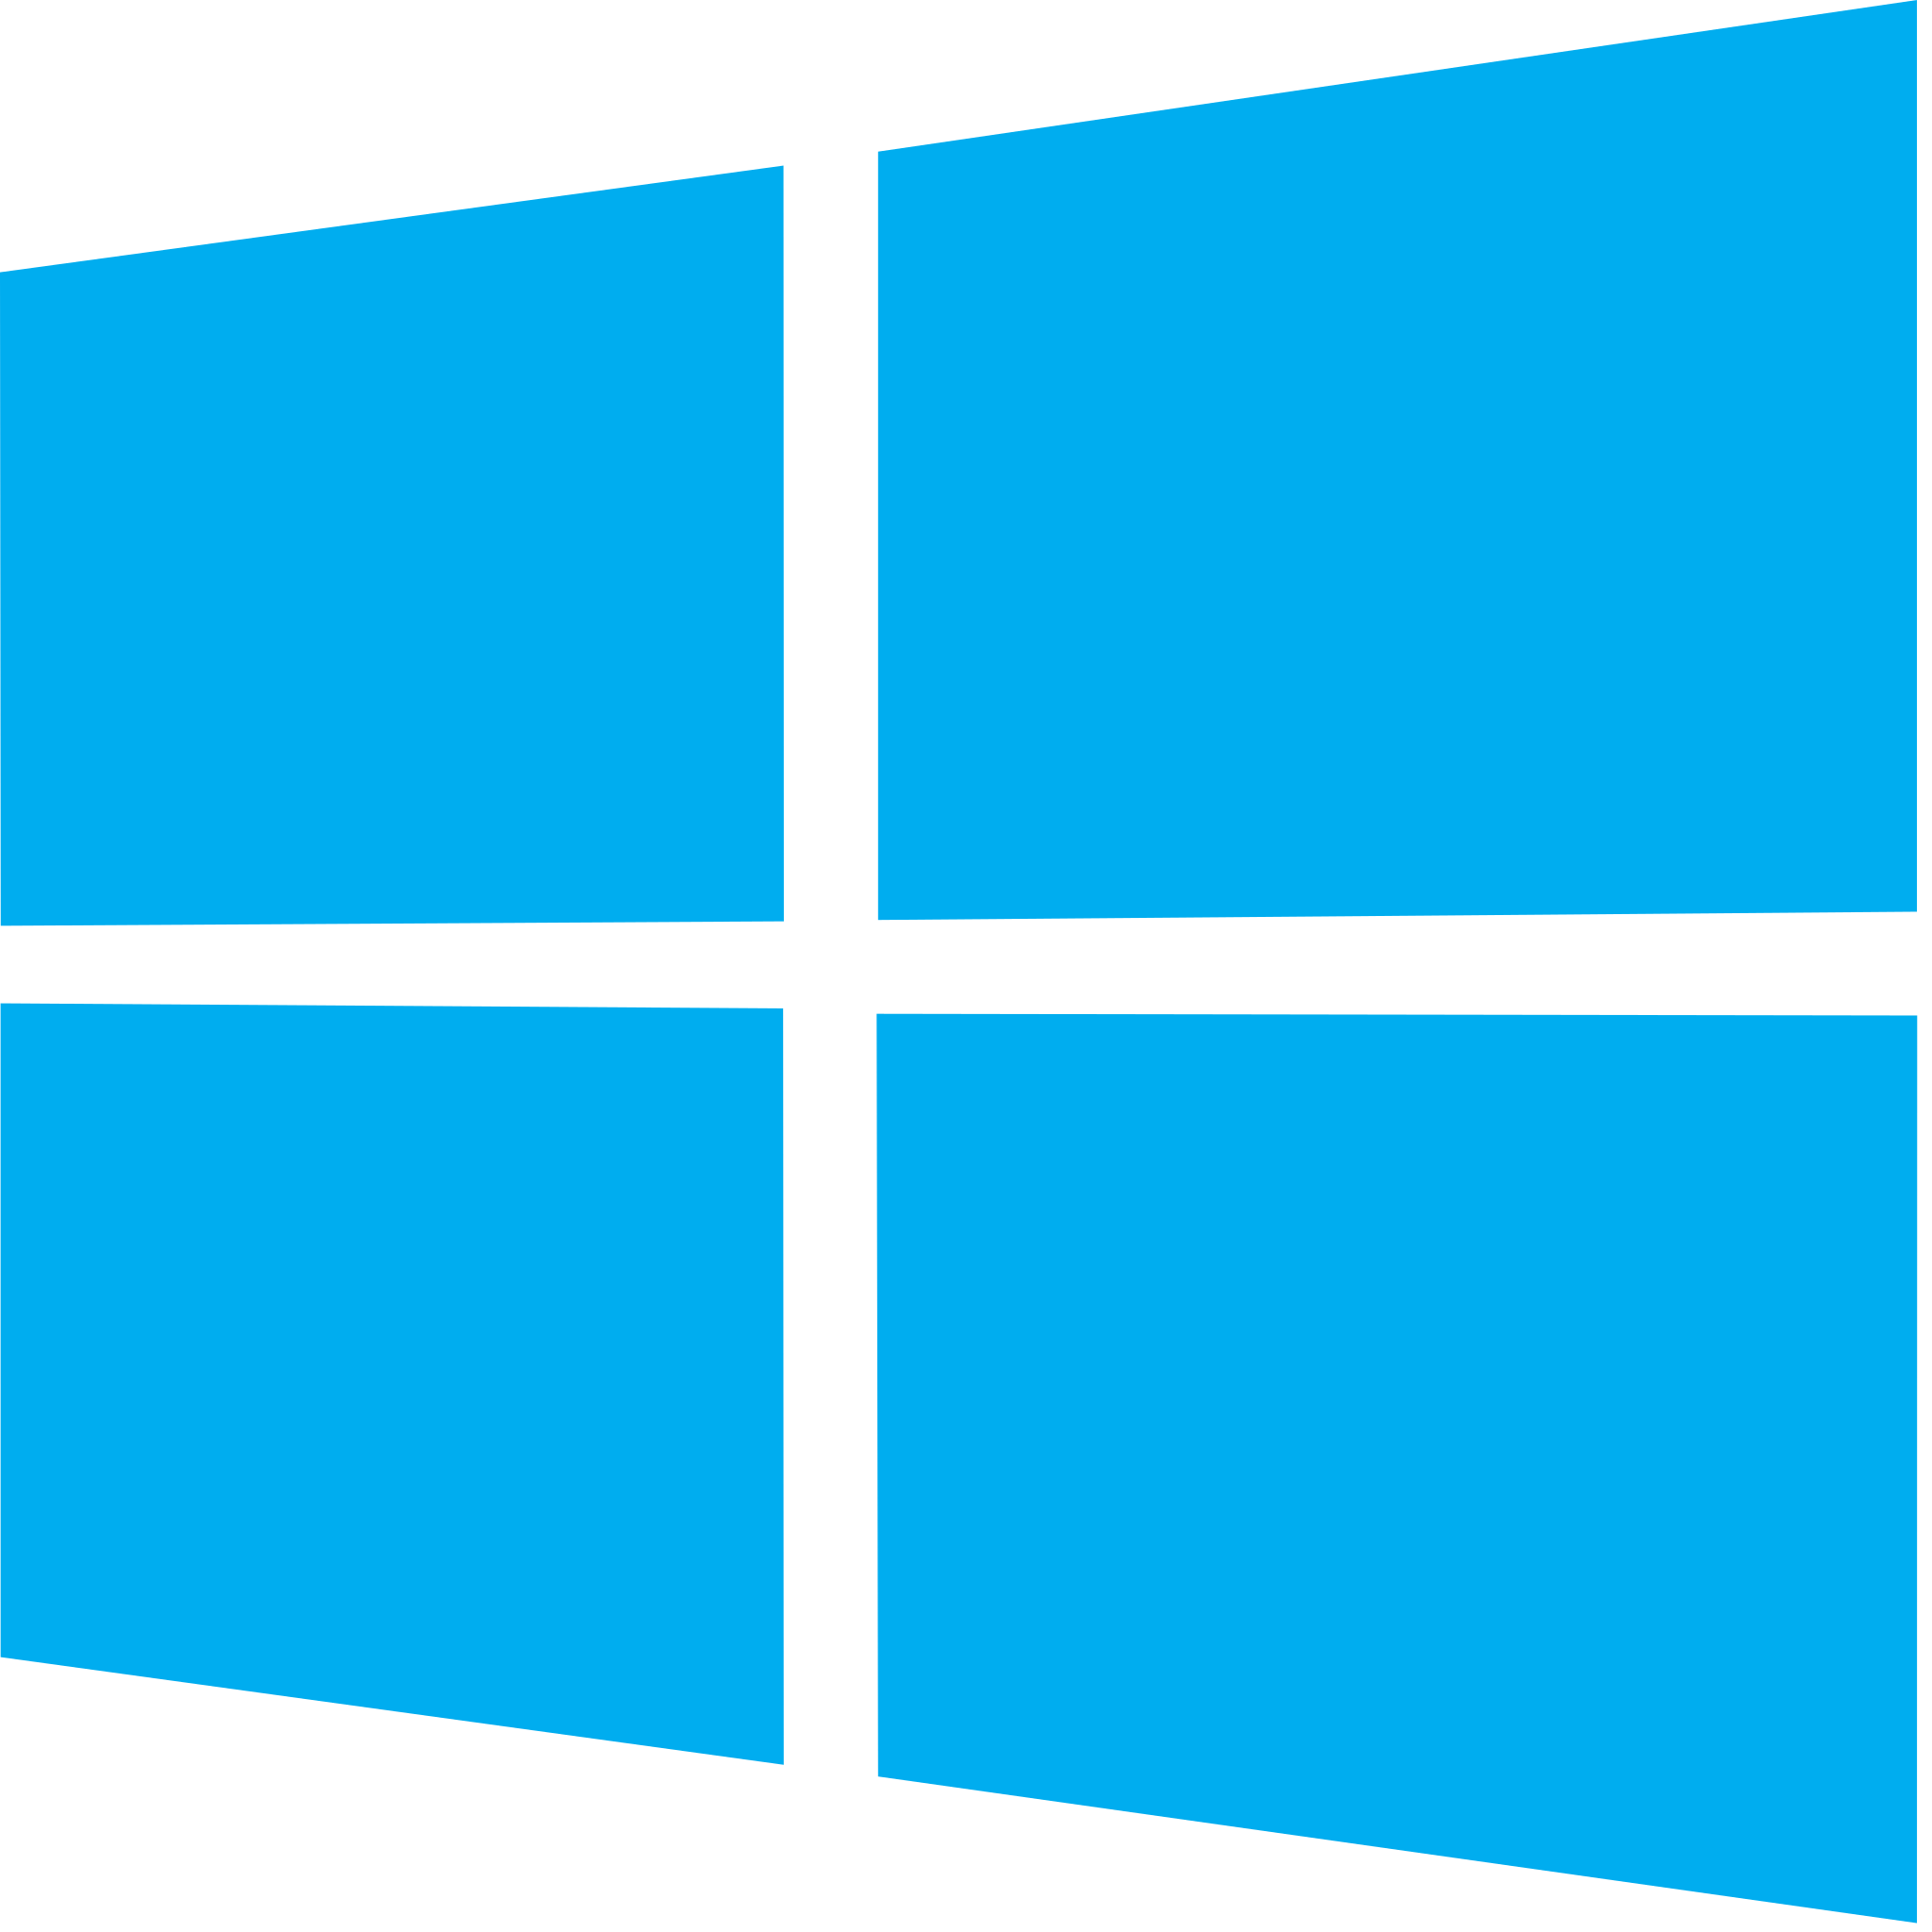
\includegraphics[width=1cm]{WindowsLogo.png}}]
	\centerline{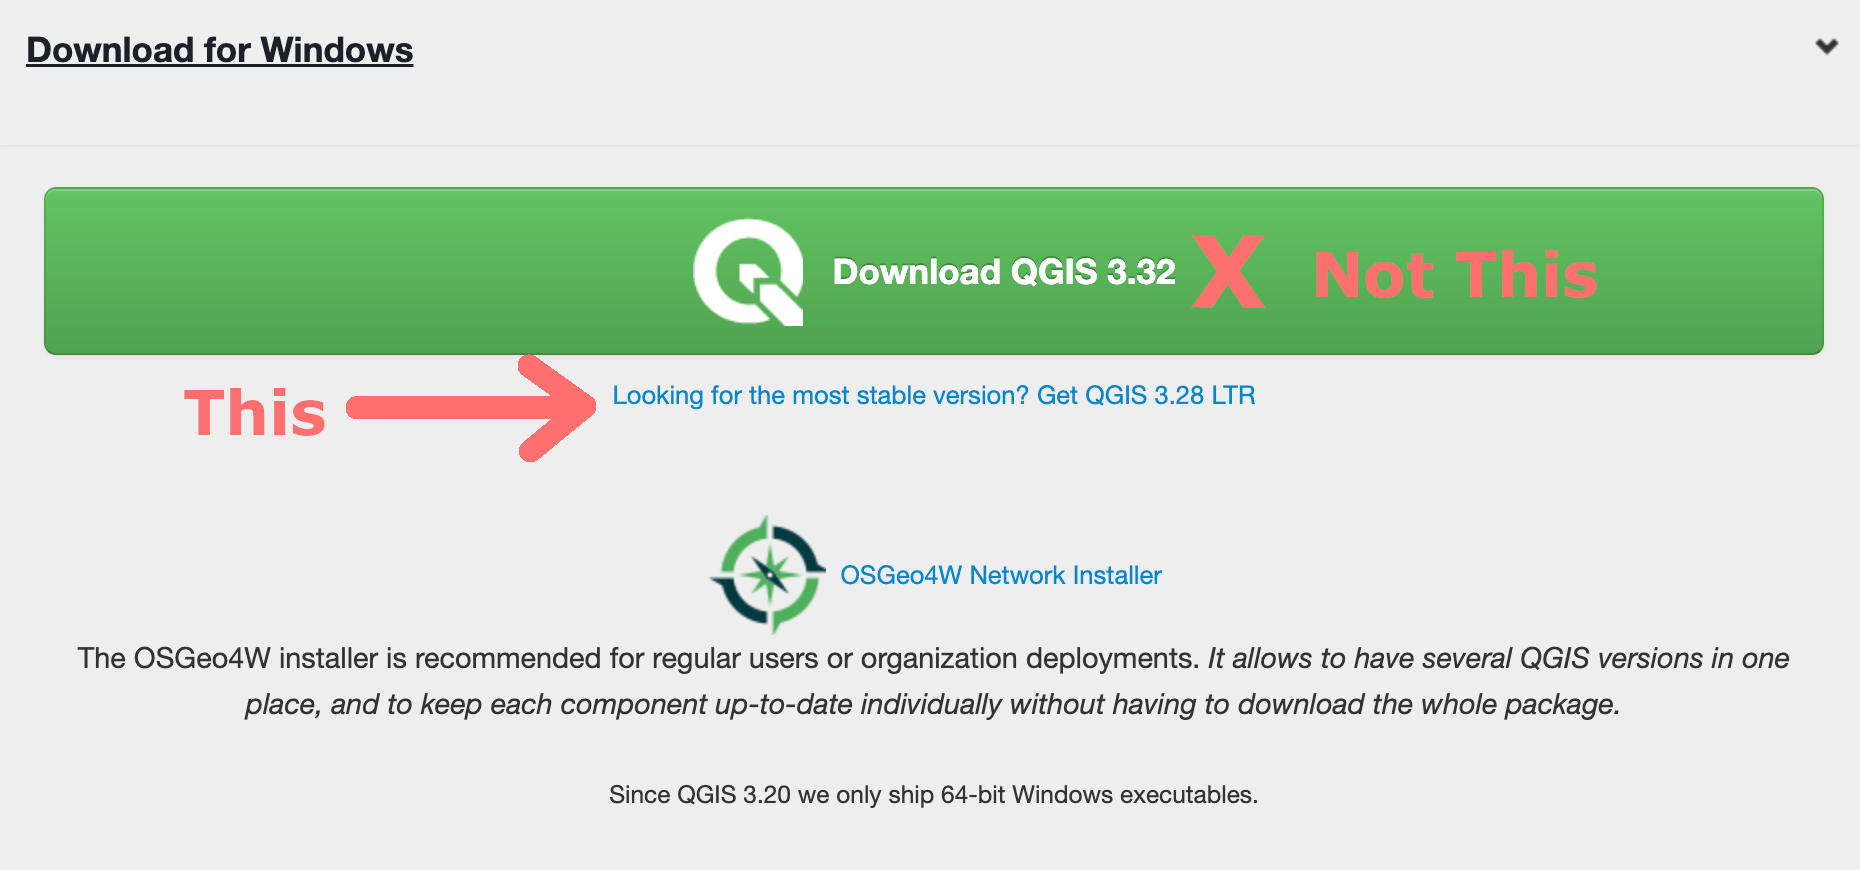
\includegraphics[width=.65\textwidth]{WINltr.png}}
	\begin{enumerate}
		\item Check for the QGIS executable file (.msi) in whichever folder you downloaded it to and open it. Follow the prompts to install the software.
		\item Open QGIS Desktop from the start menu or desktop icon.
	\end{enumerate}
\end{tcolorbox}

\begin{tcolorbox}[colback=yellow!5!white,colframe=MACred,title=\flushright{Apple macOS \hspace{.25em} 
\includegraphics[width=1cm]{AppleLogo.png}}]
	\centerline{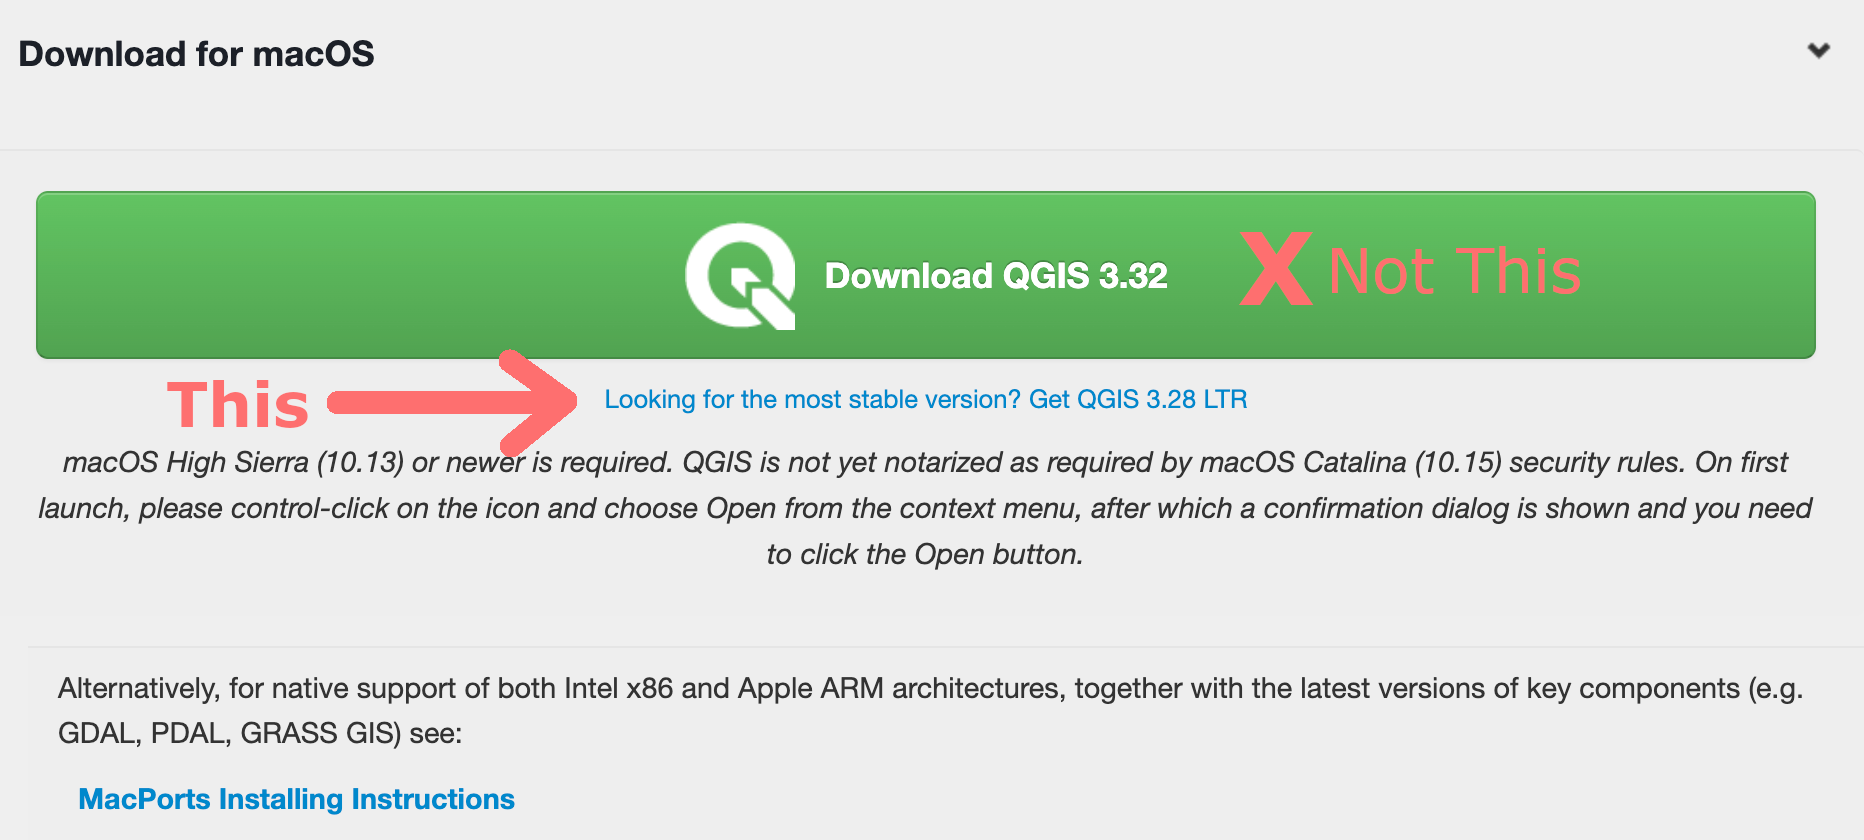
\includegraphics[width=.65\textwidth]{MACltr.png}}
	\begin{enumerate}
		\item Check for the QGIS executable file (.dmg) in whichever folder you downloaded it to and open it. Follow the prompts to accept the terms and conditions. To install the software, hold and drag the file into your Applications.
		\item Open QGIS by selecting it in Launchpad or use Go $\rightarrow$ Applications and double click on QGIS.
	\end{enumerate}
	\kulbox{\textbf{NOTE:} For MAC users, it may warn you that QGIS is not from a verifiable source. To override this problem, you can right click the app, choose ``Open'' from the menu, and then click ``Open'' in the dialog that appears. The same can be done from the toolbar. }
\end{tcolorbox}

\vspace{1em}

Congratulations! You have now successfully installed QGIS. Now attempt to open it. In our next tutorial, we will get you up and running to make your first map.

%%%%%%%%%%%%%%%%%%%%%%%%%%%%%%%%%%%%%%%%%%%%%%%%%%%%%%%%%%%%%%%%%%%%%%%%%%%%%%%%%%% End of Document
\vfill

\hrule

\vspace{1em}

\small \textbf{Recommended Citation:} Forsythe, J.D., G.R. Goldsmith, and J.B. Fisher. 2023. Observing Earth from Above Tutorials. Chapman University. \url{https://jeremydforsythe.github.io/icecream-tutorials/}

\vspace{1em}

This work is supported by funding from NASA ECOSTRESS Mission Grant \#80NSSC23K0309 (I.C.E. C.R.E.A.M.: Integrating Communication of ECOSTRESS Into Community Research, Education, Applications, and Media) and is openly licensed via \href{https://creativecommons.org/licenses/by-nc/4.0/}{CC BY-NC}.

\end{document}
